\chapter{\label{ch:3-gb-result}Understanding population structure in Africa using GhostBuster}

\minitoc

\section{Chapter overview}

In this chapter, we apply GhostBuster to real genetic data from the Human Genome Diversity Project (HGDP) and the $1{,}000$ Genomes Project ($1{,}000$ GP) to better understand the evolutionary history of humans in Africa. The chapter is divided into two main sections based on the type of event we discuss.

In Section \ref{sec:ch3-gb-bta}, we find evidence for back-to-Africa migration, which introduced Eurasian ancestry into Africa. We estimate this event occurred approximately $5{,}000$ to $15{,}000$ years ago, contributing up to 8\% to the genetic makeup of modern-day sub-Saharan Africans. In this section, we characterize and validate the admixture event, including dating the event, identifying potential source populations, and performing independent validations such as correlating Neanderthal ancestry with Eurasian ancestry in Africa and examining mutational enrichment profiles conditioned on local ancestry. Additionally, we find signatures of adaptive introgression resulting from this back-to-Africa gene flow.

In Section \ref{sec:ch3-gb-deep}, we explore and seek to understand the complex population structure in Africa before the Out of Africa event. Consistent with existing literature, we find evidence for deep population structure in Africa, with up to four ancestral components present more than $100{,}000$ years ago. These components mixed and merged in varying proportions to form present-day African populations. We also find that some of these components show excess affinity towards Neanderthals and Denisovans and exhibit differences in PRDM9 allele types. Finally, we use the inferred local ancestry to assess PGS portability for different African components, finding better PGS portability for components that contributed extensively to the Out of Africa population.  

 
\section{Back to Africa migration}
\label{sec:ch3-gb-bta}

Present-day Africans constitute a significant portion of the global population, with approximately 1.28 billion individuals.
%
This large demography also exhibits a high level of genetic diversity, which is greater than any other human population.
%
Indeed, Africans exhibit nearly twice the average nucleotide diversity compared to their Asian and European counterparts \cite{yu2002larger}. 
%
Despite this remarkable genetic richness, our understanding of the historical narratives and evolutionary trajectories of African populations remains limited. 


Migrations from Eurasia into Africa have been identified before. 
%
In fact, North African groups such as the Mozabites, Moroccans, Tunisians, and Egyptians have a significant portion of their ancestry derived from European or Middle Eastern populations, with evidence of recent admixture occurring 500-1000 years ago \cite{price2009sensitive, hellenthal2014genetic, salter2019fine}. 
%
One of the primary barriers to migration into Africa is the vast Sahara Desert, which would have impacted migrations from Eurasia into sub-Saharan Africa.
%
However, it is well known that the Sahara underwent periodic climate cycles due to changes in Earth's orbit, transitioning between arid and humid phases. 
%
The humid phase, often referred to as the ``Green Sahara'' period, could have made migrations into and out of Africa more feasible. The last Green Sahara period occurred approximately $5{,}000$ to $11{,}000$ years ago \cite{tierney2017rainfall, larrasoana2013dynamics}.

One of the first work to identify potential Eurasian ancestry in sub-Saharan Africans was conducted by Pickrell et al. \cite{pickrell2012genetic, pickrell2014ancient}.
%
They used ALDER \cite{loh2013inferring}, a method to identify and date admixture signal through coancestry curves (as described in section \ref{sec:ch1-gb-survey}) and found evidence for west Eurasian ancestry in south and east African populations, but not in West or central Africans. 
%
They estimated the proportions of west Eurasian ancestry to be up to 14\% in south African populations and up to 50\% in east African populations. These admixture events were dated to approximately 900–$1{,}800$ years ago in south Africa and $2{,}700$–$3{,}300$ years ago in east Africa. 
%
Additionally, they found the Eurasian ancestry in south Africa and east Africa to be shared and therefore theorized the most likely explanation of Eurasian ancestry in south Africa to be from east Africa.
%
While the study convincingly argued for a ``back to Africa'' migration event, the method's limited statistical power and reliance on reference populations may have hindered the detection of similar events in other African populations. 
%
These populations might have experienced smaller proportions of Eurasian ancestry or older admixture events, which were beyond the resolution of the study.

In another study, Llorente et al. \cite{llorente2015ancient} sequenced an ancient individual from the Mota caves in Ethiopia, who lived approximately 4,500 years ago. %% cite the erratum
%
This ancient DNA sample provided more direct evidence for Eurasian ancestry in African populations, as it was considered to predate the back to Africa event and thus served as a reference population without any Eurasian ancestry.
%
Using the Mota individual as a reference, the study found 4 to 7\% higher west Eurasian ancestry in east Africa, along with a much broader geographic impact of the backflow, extending to west and south Africa. 
%
They detected 7\% and 6\% Eurasian ancestry in present-day Yoruba and Mbuti individuals, respectively, populations that previously showed no signs of Eurasian ancestry and were considered ideal references for African populations. remove this sign!! %% caution!!
%
Overall, The ancient DNA provided further evidence for the backflow event affecting a wider range of African populations. However, it relied on the assumption that the ancient sample had no Eurasian ancestry, which could lead to an underestimation of Eurasian ancestry in modern African samples.
%
In fact, as we demonstrate in a later section, using our method, which does not rely on a reference population, we found some Eurasian ancestry in the Mota individual as well.

Several studies have identified small amounts of Neanderthal ancestry in African individuals, suggesting a back to Africa migration as a plausible explanation \cite{chen2020identifying,vernot2016excavating}. 
%
Chen et al. \cite{chen2020identifying} developed a novel method called IBDmix to detect introgressed Neanderthal sequences in African individuals. They discovered that modern-day Africans carry between 16.4 and 18 megabases (Mb) of Neanderthal sequence per individual, which is roughly one-third of the Neanderthal sequence found in modern-day non-Africans. 
%
Interestingly, 94\% of the Neanderthal sequences identified in African samples were shared with non-Africans, with a significantly higher overlap observed with Neanderthal sequences found in Europeans compared to East Asians.
%
The study's findings align with a model involving an ancient migration of humans to Neanderthal regions, followed by a more recent back migration to Africa. This model closely fits the observed genetic patterns.
%
Overall, the study provides independent validation of a backflow event into Africa, though it does not have the resolution to precisely characterize the proportions and timings of this event.

Finally, ancient DNA from North Africa has revealed significant migrations from the Middle East and Europe into the African continent \cite{van2018pleistocene, fregel2018ancient, simoes2023northwest}.
%
The Taforalt individual, sequenced from eastern Morocco and dated to $15{,}000$ years ago, exhibited genetic composition that was two-thirds similar to Middle Eastern hunter-gatherers and one-third similar to sub-Saharan Africans \cite{van2018pleistocene}.
%
Recent studies have uncovered additional ancient DNA in North Africa, indicating not only migrants from the Middle East but also European Neolithic farmers who introduced new lifestyles to North Africa between $7{,}000$ and $9{,}000$ years ago \cite{fregel2018ancient, simoes2023northwest}. 
%
These migrations from the Middle East and Europe likely influenced the genetics of populations throughout the rest of Africa, affecting the genetic makeup of present-day samples.


\subsection{1-8\% Eurasian ancestry in sub-Saharan African individuals}

We analyzed 17 sub-Saharan African groups across the human genome diversity project (HGDP), the 1,000 Genomes Project (1,000 GP) and Simon's genome diversity project (SGDP) and found upto 8\% Eurasian ancestry in these African populations. The groups we analyzed are listed in table \ref{tab:african_populations}a. Additionally, we also analyzed a five ancient samples in Africa, including a 8,000 year old sample from Shum Laka in Cameroon \cite{lipson2020ancient}, 2,000 and 400 year old samples from Ballito Bay, Eland Cave and Newcastle in South Africa \cite{schlebusch2017southern} and 4,500 year old sample from Mota cave in Ethiopia \cite{llorente2015ancient} (see table \ref{tab:african_populations}b). A map with all modern and ancient samples analyzed is shown in Figure \ref{fig:gb-afr-samples-map}.


\begin{table}[h!]
\centering
\begin{subtable}{\textwidth}
\centering
\resizebox{\textwidth}{!}{
\begin{tabular}{|l|l|l|c|}
\hline
\textbf{Population} & \textbf{Dataset} & \textbf{Location} & \textbf{Samples} \\ \hline
Esan & $1{,}000$GP & Nigeria & 20 \\ \hline
Gambian & $1{,}000$GP & Gambia & 20 \\ \hline
Luhya & $1{,}000$GP & Kenya & 20 \\ \hline
Mende & $1{,}000$GP & Sierra Leone & 20 \\ \hline
Biaka & HGDP & Central African Republic & 22 \\ \hline
Mandenka & HGDP & Senegal & 21 \\ \hline
Mbuti & HGDP & Democratic Republic of Congo & 12 \\ \hline
San & HGDP & Namibia and South Africa & 6 \\ \hline
Yoruba & HGDP & Nigeria & 21 \\ \hline
Bantu Kenya & HGDP & Kenya & 11 \\ \hline
Bantu SouthAfrica & HGDP & Botswana or Namibia & 8 \\ \hline
Somali & SGDP & Kenya & 2 \\ \hline
Luo & SGDP & Kenya & 2 \\ \hline
Masai & SGDP & Kenya & 2 \\ \hline
Ju Hoan North & SGDP & Namibia & 4 \\ \hline
Dinka & SGDP & Sudan & 3 \\ \hline
Khomani San & SGDP & South Africa & 2 \\ \hline
\multicolumn{3}{|l|}{\textbf{Total}} & \textbf{196} \\ \hline
\end{tabular}}
\caption{}
\label{tab:african_populations_1}
\end{subtable}

\vspace{1cm} % Adjust space between tables as needed

\begin{subtable}{\textwidth}
\centering
\resizebox{\textwidth}{!}{
\begin{tabular}{|l|l|l|l|c|}
\hline
\textbf{ID} & \textbf{Publication} & \textbf{Location} & \textbf{Coverage} & \textbf{Age} \\ \hline
I10871 & Lipson et al. \cite{lipson2020ancient} & Shum Laka, Cameroon & 18.51 & 7890 \\ \hline
new001 & Schlebusch et al. \cite{schlebusch2017southern} & Newcastle, South Africa & 11.073 & 418 \\ \hline
ela001 & Schlebusch et al. \cite{schlebusch2017southern} & Eland Cave, South Africa & 10.52 & 493 \\ \hline
baa001 & Schlebusch et al. \cite{schlebusch2017southern} & Ballito Bay A, South Africa & 12.93 & 1909 \\ \hline
I5950 & Llorente et al. \cite{llorente2015ancient} & Mota cave, Ethiopia  & 11.28 & 4472 \\ \hline
\multicolumn{4}{|l|}{\textbf{Total}} & \textbf{5} \\ \hline
\end{tabular}}
\caption{}
\label{tab:african_populations_2}
\end{subtable}

\caption{\textbf{Sub-Saharan African populations analyzed.} (a) Modern samples and, (b) Ancient samples}
\label{tab:african_populations}
\end{table}

\begin{figure}[h!]
    \centering
    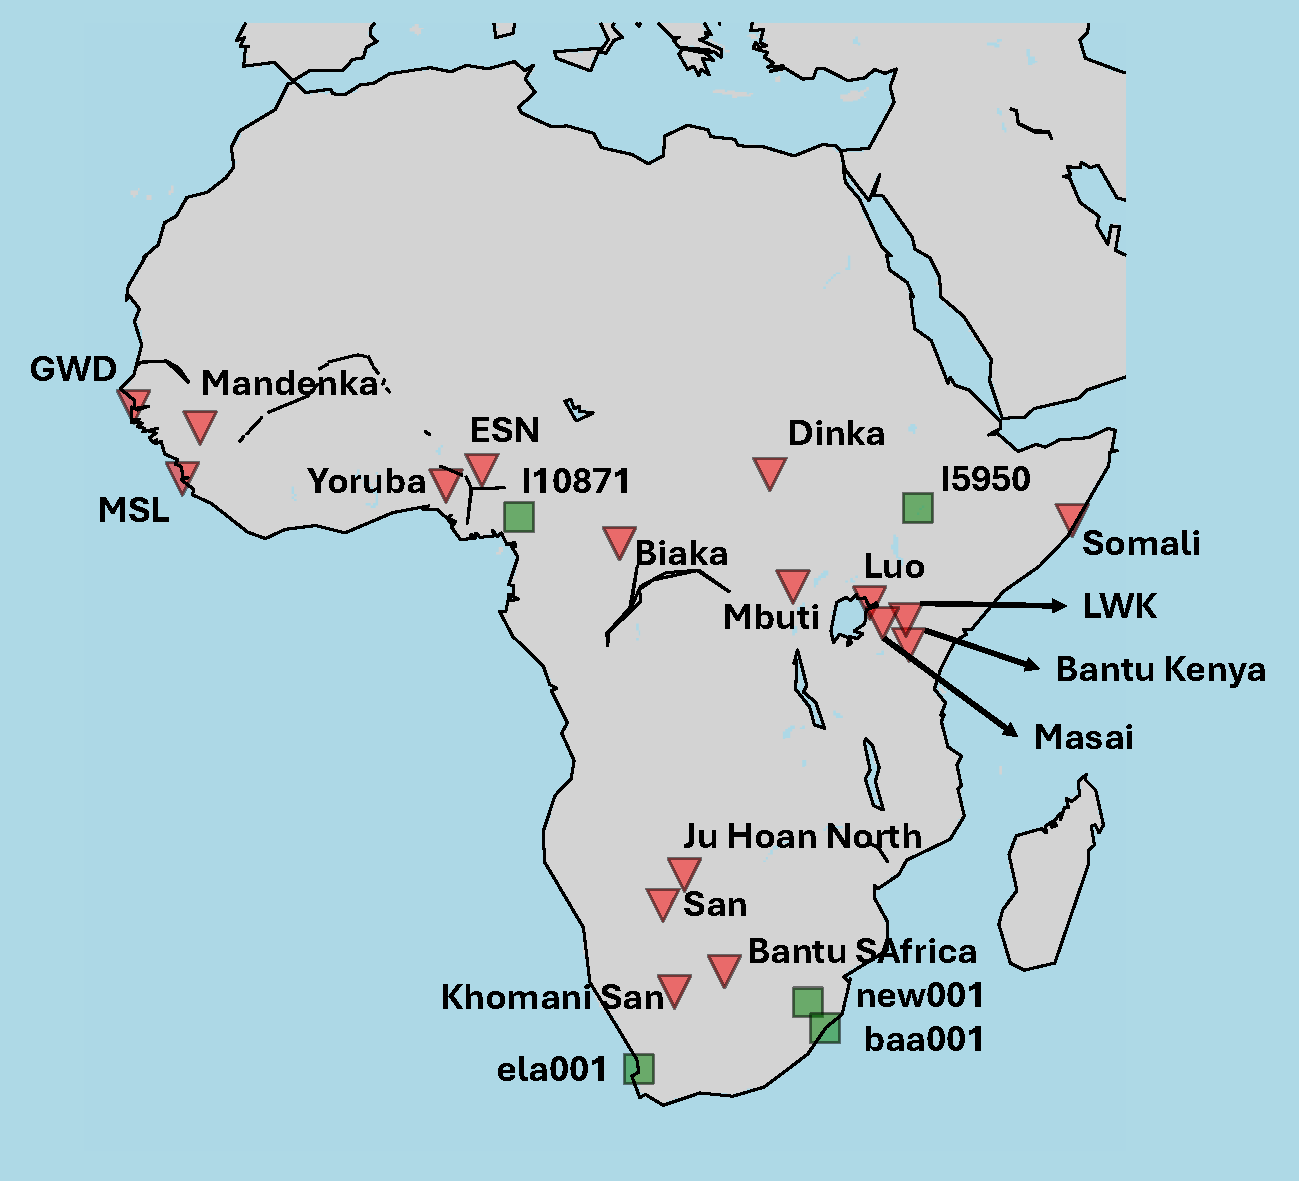
\includegraphics[width=0.75\textwidth]{figures/thesis_afr_samples.pdf}
    \caption{\textbf{Map of the African samples analyzed.} Red inverted triangles correspond to modern samples in HGDP, 1,000GP and SGDP, and green squares 5 ancient African samples.}
    \label{fig:gb-afr-samples-map}
\end{figure}

To detect Eurasian ancestry in African samples, we combined the non-Finnish Europeans (NFE), East Asians (EAS), and South Asians (SAS) in the dataset and labeled them collectively as Eurasians. Each African population was then analyzed using all Eurasians and all African populations in the dataset as reference groups. To avoid potential confounding factors, we excluded recently admixed groups such as Middle Easterners and Americans from the reference panel. We focused on coalescence events occurring between 0 and 50,000 years ago, dividing this time span into 20 epochs on a log scale, ranging from 1,000 to 50,000 years. Coalescence events after 50,000 years were disregarded, as they are likely associated with older events before the Out of Africa migration. We conducted the analysis with $k=2$ components and fixed the coalescence rates for these components based on genome-wide coalescence rates for Eurasians and the specific African population being analyzed.

We identified 1-8\% Eurasian ancestry across the modern African groups we analyzed, with the highest proportions found in the Bantu Kenyans from East Africa (xx\%) and the Mandenka from West Africa (yy\%). Among the ancient samples, we detected zz\% Eurasian ancestry in the 4,500-year-old Mota individual from Ethiopia and aa\% in the 7,900-year-old Shum Laka individual from Cameroon. In contrast, we observed little to no Eurasian ancestry in the 1,900-year-old Ballito Bay individual from South Africa, who is considered an ancestor of modern-day San individuals. These findings suggest that the back-to-Africa gene flow may have occurred earlier than previously hypothesized \cite{pickrell2012genetic,llorente2015ancient}, but may not have reached all south African population until recently. We replicated our findings using the simons genome diversity project (SGDP), which includes some African individuals from HGDP. We compared the local ancestry inferred using the SGDP reference panel with that from the HGDP+1000GP reference panel and found a high correlation in local ancestry estimates, with similar proportions of Eurasian ancestry in both datasets (see Figure aa). Additionally, we performed further analyses by adjusting the epoch boundaries and omitting the HMM, which resulted in highly correlated local ancestry and same conclusions  ($R^2 > zz$, see Figure zz). We plot the inferred Eurasian proportion for the modern and ancient samples in Figure zza and also visualize the clustering by plotting the principal components of the coalescence count matrix in Figure zzb. 


\subsection{Dating the admixture event}
%% LD-decay curves
%% Showing it was continous migration? plot the coal. time vs. segment length

We estimate the date of admixture events using coancestry curves derived from the local ancestry inferred by GhostBuster. Each African population's admixture date is estimated separately to account for population-specific variations. More detailed information on coancestry curves and their implementation can be found in Section \ref{sec:ch2-gb-coancestry}. Our analysis reveals that the timing of admixture events varies among African populations, ranging from approximately 5,000 years ago in the San to around 15,000 years ago in the Mbuti and Biaka populations. This time-range is consistent with results showing this signal in ancient African samples upto 7900 years ago. Moreover, using the radio-carbon sampling times of the ancient individuals, the admixture dates for ancient individuals also span from $xx$ to $yy$ years before present (see Figure zz).

We observe a strong negative correlation between the proportion of Eurasian ancestry and the estimated admixture date (see Figure zz), with the San population being the only outlier. Despite having the most recent admixture date, the San still exhibit a relatively low proportion of Eurasian ancestry. This pattern could likely be explained by the continuous diffusion of Eurasian ancestry from North to South Africa. As the Eurasian genetic influence moved southward, it may have been diluted by local African populations, resulting in lower proportions of Eurasian ancestry and younger admixture dates in populations further south.

%% mention about coal. time vs segment length ?

\subsection{Eurasian ancestry explains the Neanderthal ancestry in Africa}

It has been previously demonstrated that modern Africans possess small amounts of Neanderthal ancestry in their genomes, most likely due to a back-migration event from Europe \cite{chen2020identifying, bergstrom2020insights, wang2013apparent, hollfelder2017northeast}. To further explore this, we utilized GhostBuster to identify Neanderthal ancestry in African individuals by analyzing genealogies jointly inferred with modern African samples and ancient samples, including three Neanderthal samples (from Altai, Chagyrskaya and Vindija caves). Our analysis focused on coalescence events occurring between 50,000 and 1 million years ago, dividing this period into 20 epochs on a logarithmic scale. We fixed the cluster coalescence rates to that for Neanderthals and the target African population to focus on getting the Neanderthal ancestry in the sample. We performed the EM algorithm to infer the proportions, admixture times and the local ancestry of the sample. This approach provides a better way to inferring Neanderthal local ancestry in Africans, as it avoids relying on un-admixed reference samples or identity-by-descent (IBD) segments with Neanderthals, which may be biased due to human-to-Neanderthal admixture \cite{chen2020identifying}.

We find that the African samples exhibit approximately zz\% to yy\% Neanderthal ancestry, with a strong correlation between the genome-wide Neanderthal proportion and the Eurasian ancestry proportion inferred using GhostBuster ($R^2 = 0.51$, see Figure zz). The slope of the linear fit is $1.1$\%, with an intercept not significantly different from zero, suggesting that Neanderthal ancestry in these populations is closely tied to the presence of Eurasian ancestry. It also implies that the source Eurasian ancestry that contributed to back-migration event has around $1.1$\% Neanderthal ancestry. Furthermore, at the local ancestry level, we observed a $12 \times$ enrichment of Neanderthal ancestry within Eurasian segments compared to non-Eurasian segments. This significant enrichment reinforces the hypothesis that a back-migration event from Eurasia introduced the small amounts of Neanderthal ancestry in modern African samples. 

\subsection{Mutational profiles validate Eurasian segments in Africa}

There is evidence that human mutation rates have evolved over short time scales and independently across different populations \cite{harris2015evidence, harris2017rapid}. One notable example is the TCC to TTC mutation, which has been shown to be up to twice as likely to occur in Europeans compared to East Asians or Africans. 

We explore this further in the context of the back-migration event. For a given trimer, we define the normalized mutation rate per individual as the number of trimer mutations in the derived state relative to the total number of derived state mutations, considering all 96 possible trimers. We time-stratify the mutation rates into 20 epochs by accounting for allele age. For each individual in the population, we sum the numerator and denominator separately, yielding normalized mutation rates for each population. To facilitate meaningful comparisons, we further normalize these rates relative to the normalized mutation rates in African populations. This measure, termed mutation rate enrichment effectively captures the enrichment of specific mutation types in a given population compared to their normalized mutation rates in Africans. We examine this enrichment across various continental populations, including Sardinians and Basques in Europe, Han and Japanese in East Asia, and Pathans and Balochis in South Asia. Notably, we analyze the enrichment for Eurasian and non-Eurasian segments in African samples separately. We perform a chromosome-wise block-jackknife to estimate the confidence interval around the mutation rate enrichment. 

Examining the TCC to TTC mutation types, we observe significant enrichment not only in European and South Asian populations but also in the Eurasian segments within African individuals (see Figure xx). Previously, this enrichment was not detectable in Africans due to the small proportion of Eurasian segments in their genomes. However, by leveraging the local ancestry inferred using GhostBuster, we were able to isolate and identify this enrichment, providing independent validation of the back-migration event we identified. The enrichment is most pronounced in the last 20,000 years, aligning with the known evolutionary trajectory of TCC to TTC mutations, which saw a dramatic increase around 15,000 years ago and a subsequent decrease approximately 2,000 years ago \cite{harris2017rapid}. We conducted this analysis separately for each African population and consistently found significant enrichment in the Eurasian segments across all groups (see Figure xx). Populations with more recent admixture and higher proportions of Eurasian ancestry exhibited the greatest enrichment, likely due to the stronger TCC to TTC signal associated with more recent Eurasian gene flow. Further, when we stratified the Eurasian segments by length, we observed that longer segments exhibited a higher amplitude of enrichment (see Figure yy). This pattern may be attributed to either higher false positive rates in shorter segments or to ongoing Eurasian gene flow that exhibits varying TCC to TTC signal over time. Notably, San individuals, who have the most recent admixture dates, showed the highest enrichment for TCC to TTC mutations among African populations, with levels nearly matching those observed in European populations and even surpassing the enrichment seen in South Asian populations. This suggests that the timing and extent of Eurasian admixture significantly influence the presence of these mutations.

In addition to examining the TCC to TTC mutations, we also investigated the enrichment of mutations related to strong-to-weak and weak-to-strong mutation types. It is well-known that gene conversion can favor GC base pairs over AT base pairs, a phenomenon known as GC-biased gene conversion \cite{duret2009biased}. Strong-to-weak mutations are defined as those where strong alleles (GC) are mutated to weak alleles (AT), while weak-to-strong mutations involve a change from AT to GC. The impact of GC-biased gene conversion is influenced by several factors, including population size. Larger population sizes typically result in stronger GC-biased gene conversion, whereas population bottlenecks can lead to a relaxation of this bias. For our analysis, we excluded CpG sites when defining strong or weak mutations (why?). This approach allows for a more accurate assessment of the mutation patterns influenced by GC-biased gene conversion across different populations. Similar to Eurasian population, the Eurasian segments in Africans were also enriched for strong to weak mutations (and depleted for weak to strong mutations) relative to Africans as a whole. Interestingly, the Eurasian segments in Africans exhibit an even higher amplitude of strong-to-weak mutations compared to those in Europeans and East Asians. This suggests that the Eurasian population that contributed ancestry to Africa may have experienced an even more severe bottleneck than the population that initially migrated out of Africa (see Figure aa). 

\subsection{Identifying the source groups}

Next we sought to identify the source population that may have contributed to this back-migration event. To achieve this, we calculated the coalescence rates of the Eurasian segments within African genomes against a range of modern and ancient samples built in the genealogies. Specifically, we utilized the HGDP+1000GP+ancients dataset as described in Section \ref{sec:ch2-gb-data}, focusing on coalescence rates in the recent past, spanning xx to yy years ago. Additionally, we decompose each African population separately as they might not share the same source population, helping us with a more nuanced understanding of the back-migration event.

%% Para 1
% We find Bedouin, Mozabite and Sardinians to be among the most quickly coalescing populations among the modern samples, whereas Farmers in ancient groups coalesced much faster with the Eurasian segments than other European ancients.
% african ancestry in bedouin and sardinian handled?
% Sardinians more in the past, bedouin more in the recent
% how it aligns with ancients in north africa
% within africa differences? 

%% Para 2
% Overlap of Eurasian ancestry across different African populations ? - Interesting (a greedy algorithm to explain the pattern)
% relate to continous gene-flow model
% calculate p(eur in west africa | eur in east africa) or p(eur in south africa | eur in east or west africa)


\subsection{Signatures of positive selection} 

Finally, we investigate signatures of selection for specific ancestries following the admixture event by identifying regions with significantly elevated Eurasian ancestry. Due to the relatively small proportion of Eurasian ancestry in these populations, our power to detect regions with a deficit of Eurasian ancestry (Eurasian ancestry deserts) is limited. Therefore, we focus on regions where Eurasian ancestry is significantly enriched in African samples. n particular, we focus on the top 20 regions which exhibit the highest average Eurasian ancestry, with values exceeding 19\%, compared to the genome-wide average of just xx\%. These regions may highlight areas of positive selection where Eurasian alleles have been advantageous in the African populations, possibly relating to adaptive admixture.

In order to perform the functional analysis for these 20 regions we looked at the frequency of Eurasian ancestry in each of the African populations, proximity to coding region, nearest gene, ..
- We defined tag variants

%% ancestry deserts or enrichments 
%% not enough power to detect deserts 
%% functional analysis - tag variant, nearest gene, freq. across african populations

%% one specific location
%% tag variant functional enrichment (closeness to xx) GWAS enrichment


\section{Deep population structure in Africa}
\label{sec:ch3-gb-deep}

% Africa's importance in human population genetics
Africa is widely recognized as the cradle of modern humans. 
%
Fossil evidence of Homo sapiens dating back $300{,}000$ years \cite{day1969early,hublin2017new}, along with population genetics data showing high genetic diversity and the presence of some of the deepest population splits, supports this view.
%
Despite its significance in understanding human origins, the genetic history of Africa during the middle ($781{,}000$ to $126{,}000$ years ago) and late Pleistocene ($126{,}000$ to $11{,}700$ years ago) remains poorly understood. 
%
This is due to several challenges, including the lack of ancient DNA from the region, as the hot and humid climate hinders its preservation. And, recent demographic changes, such as back-to-Africa migrations (as discussed in section \ref{sec:ch3-gb-bta}), the Bantu expansion \cite{tishkoff2009genetic}, and European colonization which obscure the ancient signals when analyzing modern samples.

The population structure in Africa prior to the Out of Africa event has been a topic of considerable debate, with compelling evidence supporting the existence of structured populations even before humans expanded out of Africa.
%
Scerri et al. \cite{scerri2019beyond} argue that fossil data from Africa do not reflect contemporary humans emerging progressively in a single region. Instead, these fossils suggest that humans appeared at different times and in various combinations, exhibiting diverse ancestral features. This view is bolstered by evidence of polycentric origins of modern cognition and paleo-climatic models indicating periodic climate fluctuations.
%
The structured African metapopulation model proposed by Scerri et al. challenges the simple tree-like model of human evolution. This model suggests that ancient populations could coalesce, split, experience gene flow, or go extinct over time. Scerri et al. found that the structured metapopulation model, also referred to as the ``population fragmentation and coalescence model'', better explains the genetic and archaeological data compared to a simple panmixia model, which assumes a single, interbreeding population.

There has also been considerable research showing evidence for unsampled or `ghost' archaic hominids in Africa \cite{ragsdale2019models,hammer2011genetic,lorente2019whole,durvasula2020recovering}. For instance, Durvasula et al. employed the conditional site frequency spectrum (CSFS) to identify an archaic component in West Africans which diverged from modern humans more than $700{,}000$ years ago and contributed up to 19\% to the genetic makeup of present-day West African populations recently. Although its claims, archaic introgression in Africa is still debated as methods fail to account for the possibly complex population structure in Africa.
%
Despite these debates, African populations exhibit far more long genetic branches than non-African populations, with an average of $42{,}434$ mutations in Africans compared to $7{,}012$ in non-Africans. This suggests more complex population dynamics, either due to archaic introgression or isolation by distance \cite{speidel2019method}.

Hollfelder et al. \cite{hollfelder2021deep} and Ragsdale et al. \cite{ragsdale2023weakly} argue that the model of archaic admixture in Africa does not fully explain the genetic diversity of present-day African populations. Ragsdale et al. applied a maximum likelihood framework to infer demographic parameters that best explain the one- and two-locus statistics for various African groups. They found that the ``population fragmentation and coalescence model'' \cite{scerri2019beyond} consistently outperformed other models, including those involving archaic admixture in Africa. The proposed model by Ragsdale et al. describes a weakly structured stem, with three co-existing stem populations more than $100{,}000$ years ago. These populations underwent migration among themselves and eventually merged in different proportions to form present-day African populations. The model proposed better fits the archaeological data around that time but still suffers from model mis-specification as it constrains the possibility of models while inferring the demographic parameters.

Ancient DNA in Africa is scarce due to poor preservation in hot and humid conditions, but there are a few samples spanning the past $18{,}000$ years. Lipson et al. \cite{lipson2022ancient} argue that analyzing these ancient samples helps reduce confounding factors from more recent events such as back-to-Africa migrations, the Bantu expansion, and European colonization. By studying the ancient DNA of 31 samples, they aimed to understand the population structure of hunter-gatherers in central and southern Africa, which represent some of the deepest splits in modern human lineages. Using supervised PCA, the researchers categorized the ancient samples based on three modern African groups: the San from southern Africa, the Mbuti from central Africa, and the Dinka from northeastern Africa. They found increasing regionalization among the ancient samples, with genetic similarities best predicted by geographic locations, suggesting minimal long-range migrations within these groups. The observed patterns of variation in the ancient samples were best explained by admixture involving at least three ancestries between $20{,}000$ and $50{,}000$ years ago.

Finally, Cousins et al. \cite{cousins2024structured} provide statistical evidence for archaic admixture events that potentially affected all human populations. They propose a novel method based on the pairwise sequentially Markovian coalescent (PSMC) to identify events of population splits and mergers. Their analysis suggests that human populations underwent an admixture event approximately 300,000 years ago with two deeply divergent human species, which diverged around 1.5 million years ago. The admixture proportions in all analyzed human populations were roughly 80:20.

\subsection{A deep admixture event present in all sub-Saharan Africans}

%% 2-way, 4-way

\subsection{Joint-analysis of all sub-Saharan Africans}

%% joint-analysis

\subsection{One of the component contributed its ancestry to Neanderthals}

%% human in neaderthal? 

\subsection{Difference in PRDM9 gene across African ancestries}

%% PRMD9-C SNP
%% PRDM9 heat vs. c->t mutation rate

\subsection{Out-of-Africa component and its impact on PGS portability}

%% ANCHOR analysis

\section{Discussion}
\subsection{Limitations and future work}
- Low coverage ancients and threading
\subsection{Understanding admixtures in non human organisms}